\chapter{Preliminaries}\label{chap:preliminaries}

\section{SAT basics}

\subsection{Satisfiability problem}
A \emph{Boolean variable}, or \emph{propositional variable}, is a variable that
has two possible values : true or false (noted respectively $\true$ or $\false$).
A \emph{literal} $l$ is a propositional variable or its
negation. For a given variable $x$, the positive literal is represented by $x$
and the negative one by $\neg x$.
A \emph{clause} $\omega$ is a finite disjunction of literals represented
equivalently by $\omega = \bigvee_{i=1}^k l_i$ or the set of its literals
$\omega = \{l_i\}_{i \in \llbracket 1,k \rrbracket}$. A clause with a single
literal is called \emph{unit clause}.
A \emph{conjunctive normal form (CNF) formula} $\varphi$ is a finite
conjunction of clauses.  A CNF can be either noted $\varphi = \bigwedge_{i=1}^k
\omega_i$ or $\varphi = \{\omega_i\}_{i \in \llbracket 1,k \rrbracket}$. We
denote $\Vars_\varphi$ ($\Lits_\varphi$) the set of variables (literals) used in
$\varphi$ (the index in $\Vars_\varphi$ and $\Lits_\varphi$ is usually omitted when
clear from context).

For a given formula $\varphi$, an \emph{assignment} of the variables of
$\varphi$ is a function $\alpha: \Vars \mapsto \{ \true, \false \}$.  As usual, $\alpha$ is
\emph{total}, or \emph{complete}, when all elements of $\Vars$ have an image by
$\alpha$, otherwise it is \emph{partial}. By abuse of notation, an assignment is
often represented by the set of its true literals.  The set of all (possibly
partial) assignments of $\Vars$ is noted $\Assignments(\Vars)$.

The assignment $\alpha$ \emph{satisfies} the clause $\omega$, denoted $\alpha
\models \omega$, if $\alpha \cap \omega \neq \emptyset$. Similarly, the assignment
$\alpha$ satisfies the propositional formula $\varphi$, denoted $\alpha \models
\varphi$, if $\alpha$ satisfies all the clauses of $\varphi$. Note that a
formula may be satisfied by a partial assignment. In this case, unassigned variable are called
\emph{dont care}.
A formula is said to be
\emph{satisfiable} (\sat) if there is at least one assignment that satisfies it;
otherwise the formula is \emph{unsatisfiable} (\unsat).

\subsection{An NP-complete problem}

The SAT problems is the first NP-complete algorithm as proven by Stephen Cook in 1971~\cite{cook1971complexity}.
It is also proved by Leonid Levin in 1973~\cite{4640789}, for this purpose, it was known as Cook-Levin theorem.
The proof of to show that can be found in \cite{sipser2006introduction}.
Any NP problem can be reduced to a SAT problem in polynomial time and so open one of the most important 
unsolved problem in theoretical computer science is the P versus NP problem.
This question is one of the seven millennium prize problems.


%It asks if every problems can be solved and verified in polynomial time.
%Any NP problems can be reduced in polynomial time by a deterministic Turing machine to the SAT problems.
%The states that the propositional satisfiability problem is NP-complete
%SAT is NP because any assignment of Boolean values to Boolean variables that is claimed to 
%satisfy the given expression can be verified in polynomial time by a deterministic Turing machine. 
%
%


\subsection{Solving a SAT problem}

Two kinds of algorithm exists to solve satisfiability problems.
First, the \emph{incomplete} algorithm which does not provide any guarantee that will eventually report either any satisfiable assignment or declare that formula is unsatisfiable. This kind of algorithm is out of scope of this thesis. 
Second, the \emph{complete} algorithm, which provides a guarantee that if an assignment exists
it will be reached or it will declare that formula is unsatisfiable.
This section describes different \emph{complete }algorithm to solve a propositional formula.



\subsubsection{A naive algorithm}
A naive approach to solve a SAT problem is to try all possible assignments. In total,
for a propositional formula with $n$ variables, it leads to $2^n$ assignments in the worth case.  
\Cref{fig:naive_algo} illustrate the search tree for a given problem with six variables.
In this case $\alpha_{11}$ ($\neg x_1, \neg x_2, x_3, \neg x_4, x_5, \neg x_6 $) is found as a solution of the problem. In the general case,
this algorithm is obviously intractable on real problems even for a formula with few variables.


\begin{figure}[H]
	\centering
	
\begin{minipage}[c]{0.6\linewidth}
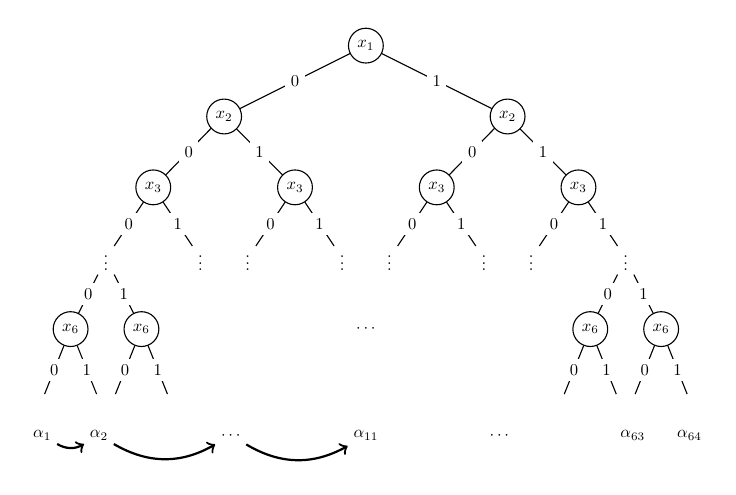
\begin{tikzpicture}[level/.style={sibling distance=60mm/#1},every node/.style={scale=0.6}, scale=0.6]
  \tikzstyle{trans}=[thick, ->, sloped]

\node [circle,draw] (x1) {$x_1$}
  child {node [circle,draw] (x2_1) {$x_2$}
    child {node [circle,draw] (x3_1) {$x_3$}
      child {node  (xn_1) {$\vdots$}
        child {node [circle,draw] (x6_1) {$x_6$}
        	child {node (x6_1f) {}
        	child[level distance=0.75cm] { node (a1) {$\alpha_1$} edge from parent[draw=none]}
        }
       		child {node (x6_1t) {}
       			child[level distance=0.75cm] { node (a2) {$\alpha_2$} edge from parent[draw=none]}
         }}
        child {node [circle,draw] (x6_2) {$x_6$}
        		child {node (x6_2f) {}}
        				child {node (x6_2t) {}
        	}
        }
      } 
      child {node (xn_2) {$\vdots$}}
    }
    child {node [circle,draw] (x3_2) {$x_3$}
      child {node (xn_3) {$\vdots$}}
      child {node (xn_4) {$\vdots$}}
    }
  }
  child {node [circle,draw] (x2_2) {$x_2$}
    child {node [circle,draw] (x3_3) {$x_3$}
      child {node (xn_5) {$\vdots$}}
      child {node (xn_6) {$\vdots$}}
    }
  child {node [circle,draw] (x3_4) {$x_3$}
    child {node (xn_7) {$\vdots$}}
    child {node (xn_8) {$\vdots$}
      child {node [circle,draw] (x6_3) {$x_6$}
      	       child {node (x6_3f) {}}
      	child {node (x6_3t) {}
        }}
      child {node [circle,draw] (x6_4) {$x_6$}
      	child {node (x6_4f) {}
        child[level distance=0.75cm] { node (an_1) {$\alpha_{63}$} edge from parent[draw=none]}
    	}
	    child {node (x6_4t) {}
    		child[level distance=0.75cm] { node (an) {$\alpha_{64}$} edge from parent[draw=none]}
      }}}
  }
};

\path (x6_2) -- (x6_3) node (x) [midway] {$\cdots$}
        child[level distance=2.25cm] { node (a_11) {$\alpha_{11}$} edge from parent[draw=none]};


\path (a2) -- (a_11) node (b1) [midway] {$\cdots$};
\path (a_11) -- (an_1) node (b2) [midway] {$\cdots$};

\draw[trans] (a1) to [bend right]  (a2);
\draw[trans] (a2) to [bend right]  (b1);
\draw[trans] (b1) to [bend right]  (a_11);

% to [bend right]  (b1) to [bend right]  (a_11);

\path (x1)   -- (x2_1) node [midway, fill=white] {$0$};
\path (x2_1) -- (x3_1) node [midway, fill=white] {$0$};
\path (x3_1) -- (xn_1) node [midway, fill=white] {$0$};
\path (xn_1) -- (x6_1) node [midway, fill=white] {$0$};
\path (x3_2) -- (xn_3) node [midway, fill=white] {$0$};
\path (x2_2) -- (x3_3) node [midway, fill=white] {$0$};
\path (x2_2) -- (x3_4) node [midway, fill=white] {$1$};
\path (x1)   -- (x2_2) node [midway, fill=white] {$1$};
\path (xn_1) -- (x6_2) node [midway, fill=white] {$1$};
\path (x3_1) -- (xn_2) node [midway, fill=white] {$1$};
\path (x2_1) -- (x3_2) node [midway, fill=white] {$1$};
\path (x3_2) -- (xn_4) node [midway, fill=white] {$1$};
\path (x3_3) -- (xn_5) node [midway, fill=white] {$0$};
\path (x3_3) -- (xn_6) node [midway, fill=white] {$1$};
\path (x3_4) -- (xn_7) node [midway, fill=white] {$0$};
\path (x3_4) -- (xn_8) node [midway, fill=white] {$1$};
\path (xn_8) -- (x6_3) node [midway, fill=white] {$0$};
\path (xn_8) -- (x6_4) node [midway, fill=white] {$1$};


\path (x6_1) -- (x6_1f) node [midway, fill=white] {$0$};
\path (x6_1) -- (x6_1t) node [midway, fill=white] {$1$};

\path (x6_2) -- (x6_2f) node [midway, fill=white] {$0$};
\path (x6_2) -- (x6_2t) node [midway, fill=white] {$1$};

\path (x6_3) -- (x6_3f) node [midway, fill=white] {$0$};
\path (x6_3) -- (x6_3t) node [midway, fill=white] {$1$};

\path (x6_4) -- (x6_4f) node [midway, fill=white] {$0$};
\path (x6_4) -- (x6_4t) node [midway, fill=white] {$1$};

\end{tikzpicture}
\end{minipage}
\begin{minipage}[c]{0.23\linewidth}
           \footnotesize
		\begin{itemize}
			\item[] $\omega_1 = \{x_1, x_2, x_3\}$ 
			\item[] $\omega_2 = \{x_4, x_5, x_6\}$
			\item[] $\omega_3 = \{\neg x_1, \neg x_5\}$
			\item[] $\omega_4 = \{\neg x_2, \neg x_4\}$
			\item[] $\omega_5 = \{\neg x_3, \neg x_4\}$
			\item[] $\omega_6 = \{\neg x_3, \neg x_6\}$
		\end{itemize}
\end{minipage}

	\caption{All possible assignments for a problem with 6 variables}
	\label{fig:naive_algo}
\end{figure}

%\hakan{Parler du DP}

\subsubsection{Davis Putnam Logemann Loveland (DPLL) algorithm}

One of the first non memory intensive algorithm to solve the SAT problems is 
the Davis Putnam Logemann Loveland (DPLL) algorithm~\cite{dpll_62}. 
It explores a binary tree using depth first search as given in \Cref{algo:dpll}.
The construction of the tree is related to a \emph{decision} literal (\cref{algo:dpll:decision}) then,
recursive call with each value are checked.
When a leaf report \unsat (\cref{algo:dpll:unsatbranch}), other branches are explored.
By recursive construction of the algorithm, when positive and negative value of a literal reach \unsat,
solver backtracks at most one level, this fact is called \emph{chronological backtracking}.
If all leaves report \unsat the formula $\varphi$ is unsatisfiable.
And so  if any branch found a solution  i.e. the problem is empty,
formula is satisfiable corresponding assignment is returned (\cref{algo:dpll:sat1,algo:dpll:sat2})

\begin{algorithm}[!htbp]
	\SetKwProg{Fn}{function}{}{}
	\SetKwFunction{DPLL}{DPLL}	
	\SetKwFunction{unitPropagation}{unitPropagation}
	\SetKwFunction{purePropagation}{purePropagation}
	\SetKwFunction{assignDecisionLiteral}{assignDecisionLiteral}

	
	\Fn{
		\DPLL{$\varphi$: CNF formula, $\alpha$ assignment}\\
		$\quad\quad$\textbf{returns} an assignment if $\varphi$ is \sat and $\unsat$ otherwise
	}
	{	
		$\varphi, \alpha \gets$ \unitPropagation{$\varphi, \alpha$}\;
	\label{algo:dpll:unit}
		\If{$\{\} \in \varphi$}{\Return \false \tcp*{Conflict}}	 \label{algo:dpll:unsatbranch}
		
		\If{$\varphi = \{\}$}{\Return $\alpha$ \tcp*{$\varphi$ is $\sat$}}
		
		$x \gets$ \assignDecisionLiteral{}\; \label{algo:dpll:decision}

		\If{$\alpha \gets$ \DPLL{$\varphi \cup \{x\}, \alpha $} \label{algo:dpll:pos}} 
		{
			\Return $\alpha$ 		\label{algo:dpll:sat1}
		}
		\If{ $\alpha \gets$ \DPLL{$\varphi \cup \{\neg x\}, \alpha $} \label{algo:dpll:neg}}
		{
			\Return $\alpha$ 		\label{algo:dpll:sat2}
		} 
	
		\Return \unsat \tcp*{$\varphi$ is $\unsat$}\label{algo:dpll:unsat}
	}
	\caption{The DPLL algorithm.}
	\label{algo:dpll}
	
\end{algorithm}

An important function in the DPLL algorithm is \texttt{unitPropagation} \cref{algo:dpll:unit} and
it is detailed in \Cref{algo:unitdpll}. It searches all unit clauses to ensure satisfiability,
negative literals are removed from the clause that belongs to him. Then, given formula is either simplified
or leads to an inconsistency (empty clause). Unit literals are also added to the current assignment.

\begin{algorithm}[!htbp]
	\SetKwProg{Fn}{function}{}{}
	\SetKwFunction{unitPropagation}{unitPropagation}
	\Fn{
		\unitPropagation{$\varphi$: CNF formula, $\alpha$ assignment}\\
		$\quad\quad$\textbf{returns}  CNF formula and assignment $\alpha$ 
	}
	{	
		\While{$\{l\} \in \varphi$ \textbf{and} $\{\} \notin \varphi$  }
		{
			\tcp{\small Remove all clauses containing $l$, all literals $\neg l$}
			$\varphi \gets \varphi\mid_{\,l}$\\
			$\alpha \gets \alpha \cup \{l\}$

		}
	\Return $\varphi, \alpha$
	}
	\caption{Unit propagation}
	\label{algo:unitdpll}
	
\end{algorithm}

When DPLL algorithm is executed on the formula in \Cref{fig:naive_algo}, unit propagation prevents to 
explore assignments from $\alpha_1 $ to $\alpha_{8}$. Moreover, application to unit propagation until fix point
leads directly to the solution. 
An important part of efficiency of DPLL is \texttt{assignDecisionLiteral} . The objective of this function 
is to find a literal that will generate a maximum of unit propagation. Intuitively, decision literals 
can be viewed as "guesses" and propagated literals can be viewed as "deductions". Finding a optimal variable
is NP-Hard \cite{biere2009handbook}. Different heuristics exists, one of them will be presented in 
\hakan{CITE SECTION DECISION HEURISTICS}.


%\input{algo/puredpll}
%Another idea introduced by DPLL was \emph{elimination of pure literals},
%a literal is said pure if it only appear on one sign (positive or negative) in the problem.
%These literals are set to true in the assignment.
%On consequence, all clauses that own these literals are satisfied and so can be removed.
%
\subsubsection{Conflict Driven Clause Learning (CDCL) algorithm}

The principal weakness of DPLL algorithm is to make same inconsistencies several times
(principally due to chronological backtracking), incurring unnecessary CPU usage.\\
Conflict Driven Clause Learning (CDCL) \cref{algo:cdcl} is another sound and complete algorithm
to resolve a SAT problem and overcome its principal weakness.


\Cref{algo:cdcl} gives an overview of CDCL, Like DPLL,  it walks a binary search tree.
It first applies unit propagation to the formula $\varphi$ for the current assignment $\alpha$ (\cref{alg:cdcl:unit}).
Note that it is exactly the same procedure as the one used for DPLL.
An inconsistency or a \emph{conflict} at level $0$ indicates that the formula is not satisfiable, and the algorithm
reports it (\cref{alg:cdcl:unsat_start,alg:cdcl:unsat_end}). When the conflict is occurring at a higher level, it
reason was analyzed and a clause called \emph{conflict clause} is deduced (\cref{alg:cdcl:analyze}).
 This clause is \emph{learnt} (\cref{alg:cdcl:learn}), as it does not change the
satisfiability of $\varphi$, and avoids encountering a conflict with the same
causes in the future. This function will be presented thereafter
The analysis is completed by the computation of a backjump point to which the algorithm backtracks (\cref{alg:cdcl:backjump}).
Finally, if no conflict appears, the algorithm chooses a new decision literal 
(\cref{alg:cdcl:pick_start,alg:cdcl:pick_end}).
The above steps are repeated until the satisfiability status of the
formula is determined.


\begin{algorithm}
	\SetKwProg{Fn}{function}{}{}
	\SetKwFunction{CDCL}{CDCL}
	\SetKwFunction{unitPropagation}{unitPropagation}
	\SetKwFunction{analyzeConflict}{analyzeConflict}
	\SetKwFunction{addLearntClause}{addLearntClause}
	\SetKwFunction{assignNewLiteral}{assignDecisionLiteral}
	\SetKwFunction{backjumpPolicy}{backjumpAndRestartPolicies}
	\SetKwFunction{ca}{currenttAssignment}
	\Fn{
		\CDCL{$\varphi$: CNF formula}\\
		$\quad\quad$\textbf{returns} $\true$ if $\varphi$ is \sat and $\false$ otherwise
	}
	{
		$dl \gets 0$ \tcp*{Current decision level}
		$\alpha \gets \emptyset$\;
		\While{not all variables are assigned}{
			$\varphi, \alpha \gets$ \unitPropagation{$\varphi|_\alpha, \alpha$}\;\label{alg:cdcl:unit}
			\If(\tcp*[f]{A conflict occurs}){ $\{\} \in \varphi$}
			{ 
				\If{dl = 0}{\label{alg:cdcl:unsat_start} 
					\Return \false \label{alg:cdcl:unsat_end} 
					\tcp*{$\varphi$ is $\unsat$}
				}
				$\omega \gets$ \analyzeConflict{}\;\label{alg:cdcl:analyze} 
				$dl \gets$ \backjumpPolicy{}\;\label{alg:cdcl:backjump} 
				$\varphi \gets \varphi \cup \{\omega$\} \; \label{alg:cdcl:learn}
				
			}
			\Else{
				$\alpha \gets \alpha\, \cup $ \assignNewLiteral{}\; \label{alg:cdcl:pick_start} 
				$dl \gets dl+1$\;\label{alg:cdcl:pick_end} 
			}
		}
		\Return \true
		\tcp*{$\varphi$ is $\sat$}
	}
	\caption{The CDCL algorithm.}
	\label{algo:cdcl}
	
\end{algorithm}


%If a conflict is detected in higher level, it is analyzed, which provides a
%explaining the reason for the conflict.
%Different heuristics exists about the computation of conflict clause, on recent solvers
%the most used heuristic is the first Unique Implication Point ($1^{th}$ UIP) \cite{zhang2001efficient}.
%Restart is an important things in SAT solver, it allows solver to explore a new search space
%with the learned clauses. It is also finely intertwined with the decision heuristics.
%If the solver is working on "hard" part of the problem it will reconsider the decision variables and
%solve this part part at first. But if we restart too often the solver doesn't have to discover new things.
%
%
%  This clause is learnt (\cref{alg:cdcl:learn}), as it does not change the
%satisfiability of $\varphi$, and avoids encountering a conflict with the same
%causes in the future.
%
%
% The choice of the decision literal
%affect the performance of solver. The first most used heuristic is Variable State Independent Decaying Sum (VSIDS)~\cite{moskewicz2001chaff}. The idea behind this heuristic is that the "hard" parts of the search space 
%will be treated first. To do that, each variable has an activity and wa increase if it participate to the resolution
%of the conflict.
%The second most used heuristics is Learning rate based branching (LRB~\cite{liang2016learning})
%The above steps are repeated until the satisfiability status of the formula is determined.


\subsection{Conflict Analysis}
A conflict is an inconsistency discovered by the solver, a situation that requires for a variable to be set 
simultaneously to the \true and \false value. \Cref{fig:conflict} shows an assignments that leads to a conflict.
First the solver chose $\neg x_1$ as decision then $\neg x_6$ and then $\neg x_5$. This last one propagates $x_4$
which in turn propagates $x_2$ and $x_3$. On clause $\omega_1$, $x_3$ needs to be true and false in $\omega_5$ so
a conflict appears.
 
\begin{figure}[H]
	\centering
		{\scriptsize
\newcommand{\ratioc}{0.195}
%\begin{minipage}[l]{\ratioc\linewidth}
%	\begin{itemize}
%		\item[] $\omega_1 = \{\cred{x_1}, x_2, x_3\}$ 
%		\item[] $\omega_2 = \{x_4, x_5, x_6\}$
%		\item[] $\cgreen{\omega_3} = \{\cgreen{\neg x_1}, \neg x_5\}$
%		\item[] $\omega_4 = \{\neg x_2, \neg x_4\}$
%		\item[] $\omega_5 = \{\neg x_3, \neg x_4\}$
%		\item[] $\omega_6 = \{\neg x_3, \neg x_6\}$
%	\end{itemize}
%\end{minipage}
\begin{minipage}[b]{\ratioc\linewidth}
	\begin{itemize}
	\item[] $\omega_1 = \{\cred{x_1}, x_2, x_3\}$ 
	\item[] $\omega_2 = \{x_4, x_5, \cred{x_6\}}$
	\item[] $\cgreen{\omega_3} = \{\cgreen{\neg x_1}, \neg x_5\}$
	\item[] $\omega_4 = \{\neg x_2, \neg x_4\}$
	\item[] $\omega_5 = \{\neg x_3, \neg x_4\}$
	\item[] $\cgreen{\omega_6} = \{\neg x_3, \cgreen{\neg x_6\}}$
\end{itemize}
\end{minipage}
\begin{minipage}[b]{\ratioc\linewidth}
		\begin{itemize}
		\item[] $\omega_1 = \{\cred{x_1}, x_2, x_3\}$ 
		\item[] $\omega_2 = \{\cprop{x_4}, \cred{x_5}, \cred{x_6\}}$
		\item[] $\cgreen{\omega_3} = \{\cgreen{\neg x_1}, \cgreen{\neg x_5\}}$
		\item[] $\omega_4 = \{\neg x_2, \neg x_4\}$
		\item[] $\omega_5 = \{\neg x_3, \neg x_4\}$
		\item[] $\cgreen{\omega_6} = \{\neg x_3, \cgreen{\neg x_6\}}$
	\end{itemize}
\end{minipage}
\begin{minipage}[b]{\ratioc\linewidth}
			\begin{itemize}
		\item[] $\omega_1 = \{\cred{x_1}, x_2, x_3\}$ 
		\item[] $\cgreen{\omega_2} = \{\cgreen{x_4}, \cred{x_5}, \cred{x_6\}}$
		\item[] $\cgreen{\omega_3} = \{\cgreen{\neg x_1}, \cgreen{\neg x_5\}}$
		\item[] $\omega_4 = \{\neg x_2, \cred{\neg x_4}\}$
		\item[] $\omega_5 = \{\neg x_3, \cred{\neg x_4}\}$
		\item[] $\cgreen{\omega_6} = \{\neg x_3, \cgreen{\neg x_6\}}$
	\end{itemize}
\end{minipage}
\begin{minipage}[b]{\ratioc\linewidth}
	\begin{itemize}
		\item[] $\omega_1 = \{\cred{x_1}, x_2, x_3\}$ 
		\item[] $\cgreen{\omega_2} = \{\cgreen{x_4}, \cred{x_5}, \cred{x_6\}}$
		\item[] $\cgreen{\omega_3} = \{\cgreen{\neg x_1}, \cgreen{\neg x_5\}}$
		\item[] $\omega_4 = \{\neg x_2, \cred{\neg x_4}\}$
		\item[] $\omega_5 = \{\neg x_3, \cred{\neg x_4}\}$
		\item[] $\cgreen{\omega_6} = \{\neg x_3, \cgreen{\neg x_6\}}$
	\end{itemize}
\end{minipage}
\begin{minipage}[b]{\ratioc\linewidth}
	\begin{itemize}
		\item[] $\omega_1 = \{\cred{x_1}, \cred{x_2}, \cblue{x_3}\}$ 
		\item[] $\cgreen{\omega_2} = \{\cgreen{x_4}, \cred{x_5}, \cred{x_6\}}$
		\item[] $\cgreen{\omega_3} = \{\cgreen{\neg x_1}, \cgreen{\neg x_5\}}$
		\item[] $\cgreen{\omega_4} = \{\cgreen{\neg x_2}, \cred{\neg x_4}\}$
		\item[] $\omega_5 = \{\cblue{\neg x_3}, \cred{\neg x_4}\}$
		\item[] $\cgreen{\omega_6} = \{\neg x_3, \cgreen{\neg x_6\}}$

	\end{itemize}
\end{minipage}
}


	\caption{Decisions/Propagations that leads to a  conflict}
	\label{fig:conflict}
\end{figure}

This series of decisions would provoke same propagation and leads to the same conflict. To avoid this
situation, the solver needs to analyze the reason of the conflict with so called \emph{implication graph}.
Implication graph represents the current state of the solver proof system.
This graph is updated when a variable is assigned either on decision or propagation and when a variable
is unassigned.


\begin{figure}[H]
	\centering
	
\begin{tikzpicture} % [level/.style={sibling distance=60mm/#1},every node/.style={scale=0.89}, scale=0.89]

	\tikzstyle{decision}=[draw,double,circle,fill=red!25,minimum size=45pt,inner sep=0pt]
	\tikzstyle{propagation}=[draw,circle,fill=white!25,minimum size=45pt,inner sep=0pt]
	
	\node[decision] (dx1) {$\neg x_1$@1};
	\node[decision] (dx6) at ($(dx1) + (0, -2)$) {$\neg x_6$@2};
	\node[decision, draw=orange!80] (dx5) at ($(dx6) + (0, -2)$) {$\neg x_5$@3};
	
	\node[propagation, draw=orange, line width=0.5mm] (px4) at ($(dx6) + (4, -1)$) {$x_4$@3};
	\node[propagation] (px3) at ($(dx5) + (12, 0)$) {$\neg x_3$@3};
	\node[propagation] (px2) at ($(dx6) + (8, 0)$) {$\neg x_2$@3};

	\node[propagation] (px33) at ($(dx5) + (12, 4)$) {$x_3$@3};


	\node[font=\bfseries] (reason) at (2,-6) {\textcolor{orange}{Reason Side}};
	\node[font=\bfseries] (reason) at (9,-6) {\textcolor{orange}{Conflict Side}};

	\path[->, draw, thick] (dx6) -- (px4) node [midway, fill=white] {$\omega_2$};
	\path[->, draw, thick] (dx5) -- (px4) node [midway, fill=white] {$\omega_2$};
	
	\path[->, draw, thick] (px4) -- (px3) node [midway, fill=white] {$\omega_5$};
	\path[->, draw, thick] (px4) -- (px2) node [midway, fill=white] {$\omega_4$};
	
	\path[->, draw, thick] (dx1) -- (px33) node [midway, fill=white] {$\omega_1$};
	\path[->, draw, thick] (px2) -- (px33) node [midway, fill=white] {$\omega_1$};
	\path[<->, draw, line width=1mm, color=blue!60] (px3) -- (px33);
	\path[line width=0.5mm, draw=orange] ($(px4.east) + (0.5, -2)$) -- ($(px4.east) + (0.5, 4)$)  
			   node [fill=white] {\textcolor{orange}{Cut 1}};
	
%	\path[line width=0.5mm, draw=orange!60] ($(px4.east) + (-3.5, -2)$) -- ($(px4.east) + (-3.5, 4)$)
%			   node [fill=white] {\textcolor{orange!70}{Cut 2}};
	
	% Legend
	
	\path[draw] (-1, -6.5) -- (13, -6.5);
	\node[decision, scale=0.3] (ld) at (0, -7) {};
	\node[align=left, text width=2.2cm] at (1.5, -7) {Decision};
	
	\node[propagation, scale=0.3] (lp) at (0, -7.7) {};
	\node[align=left, text width=2.2cm] at (1.5, -7.7) {Propagation};
	
	\node[scale=1.5] (lz) at (5, -7) {$\rightarrow$};
	\node[align=left, text width=2.2cm] at (6.5, -7) {Implication};
	
	\node[scale=1.5] (ld) at (5, -7.7) {\textcolor{blue!60}{$\leftrightarrow$}};
	\node[align=left, text width=2.2cm] at (6.5, -7.7) {Conflict};
	
	\node[propagation, draw=orange, line width=0.5mm, scale=0.3] (le) at (10, -7) {};
	\node[align=left, text width=2.2cm] at (11.5, -7) {UIP};
	
	\node[scale=2] (ld) at (10, -7.7) {\textcolor{orange}{\textendash}};
	\node[align=left, text width=2.2cm] at (11.5, -7.7) {Cut};
	\path[draw] (-1, -8.2) -- (13, -8.2);
\end{tikzpicture}

	\caption{Implication graph}
	\label{fig:implication-graph}
\end{figure}

\subsection{Heuristics}

\textbf{Decision heuristics}. Variable used to divide problems have a huge impact on the 
overall solving time by the solver. Decision variable may impact the number of propagation and so the depth of the search tree  As propagated one can be seen as \emph{deduction} and the 




\hakan{Peut être mettre les heuristiques dans des paragraphes}

\hakan{Literal Block Distance LBD}

\section{Groups basics}

Symmetries is related to a branch of mathematics called group theory. This section give us an overview of group
theory.

\subsection{Groups}

A \emph{group} is a structure $\langle G, * \rangle$, where $G$ is a non empty set and $*$ a binary
operation such the following axioms are satisfied:
\begin{itemize}[noitemsep,nolistsep]
	\item \emph{associativity}: $\forall a, b, c \in G, (a * b) * c = a * (b * c)$
	\item \emph{closure}: $\forall a, b \in G, a * b \in G$.
	\item \emph{identity}: $\forall a \in G, \exists e$ such that $ a * e = e * a = a$
	\item \emph{inverse}:  $\forall a \in G, \exists b \in G$, commonly denoted $a^{-1}$ such that
	 $a * a^{-1} = a^{-1} * a = e$
\end{itemize}

Note that \emph{commutativity} is not required i.e $\ a * b = b * a$, for $a, b \in G$.
The group is \emph{abelian} if it satisfies the commutativity rule.
Moreover, the last definition leads to important properties which are: i) uniqueness of the identity element. 
To prove this property, assume $\langle G, * \rangle$ a group with two identity elements $e$ and $f$ 
then $ e = e * f = f$.
ii) uniqueness of the inverse element. To prove this property, suppose that an element $x_1$ has two inverses,
denoted $b$ and $c$ in group $\langle G, * \rangle$, then\\
	$\begin{array}{lcll}					
			b & = & b * e & \\
			  & = & b * (a * c) & c \text{ is an inverse of } a, \text{so } e = a * c\\
			  & = & (b * a) * c &   \text{\emph{associativity} rule}\\
			  & = & e * c       & b \text{ is an inverse of } a, \text{so } e = a * b\\
			  & = & c           &   \text{\emph{identity} rule}
	\end{array}$

The structure $\langle G, * \rangle$ is denoted as G when clear from context that G is a group
with a binary operation. In this thesis, we interested only with the \emph{finite} groups i.e
with a finite number of elements.

Given a group $G$, a \emph{subgroup} is a non empty subset of $G$ which is also a group with 
the same binary operation. If $H$ is a subgroup of $G$, we denote as $H \leq G$.
A group has at least two subgroups: i) the subgroup composed by identity element $\{e\}$, denoted \emph{trivial} subgroup. All other subgroups are \emph{nontrivial}; ii) the subgroup composed by itself, denoted \emph{improper} subgroup. All other subgroups are \emph{proper}.


\subsubsection{Generators of a group}

If every elements in a group G can be expressed as a linear combination
of a set of group of elements S = $\{g_1, g_2, ..., g_n \}$ then we say G is 
generated by the S. we denote this as G = $\langle S \rangle$ =
$\langle \{g_1, g_2, ..., g_n \} \rangle$ 



\subsection{Permutation groups}
 
A \emph{permutation} is a bijection from a set $X$ to itself.\\
 Example: given a set $X = \{x_1, x_2, x_3, x_4, x_5, x_6\}$,
$g = ${\Bigg( \begin{tabular}{cccccc}
		$x_1$ & $x_2$ & $x_3$ & $x_4$ & $x_5$ & $x_6$\\
		$x_2$ & $x_3$ & $x_1$ & $x_4$ & $x_6$ & $x_5$
	\end{tabular} \Bigg)}\\
$g$ is a permutation that maps $x_1$ to $x_2$, $x_2$ to $x_3$, $x_3$ to $x_1$, $x_4$ to $x_4$, $x_5$ to $x_6$ and $x_6$ to $x_5$.

Permutations are generally written in \emph{cycle notation} and the self mapped elements are omitted.
So the permutation in cycle notation will be : $g$ = ($x_1$ $x_2$ $x_3$) ($x_5$ $x_6$).
We say \emph{support} of the permutation $g$ noted $supp(g)$ the elements that not mapped to themselves,
$supp(g) = \{ x \in X \mid g.x \neq x\}$. A variable $x$ is \emph{stabilized} by a permutation $g$ 
if $x \notin \support(g)$. A clause $\omega$ is \emph{stabilized} by a permutation $g$ if 
$\omega \cap \support(g) = \emptyset$. \hakan{Maybe stabilisation as definition ?}


The set of permutations of a given set $X$ form a group $G$,
with the composition operation ($\circ$) and called \emph{permutation group}.
The \emph{symmetric group} id the set of all possible permutations of a set $X$ and noted \Group($X$).
%The set of \textbf{all} permutations of a set $X$ is the \emph{symmetric group} of $X$ and noted \Group($X$).
So, a \emph{permutation group} is a subgroup of \Group($X$). 
%A set of permutations $P$ is a set of \emph{generators} of a group $G$ if each permutation of $G$
%can be expressed as a composition of permutations in $P$. 


A permutation group $G$ induces a \emph{equivalence relation} on the set of element $X$ being
permuted. Two elements $x_1, x_2 \in X$ are equivalent if there exists a permutation $g \in G$ such that
$g x_1 = x_2$. Then equivalence relation partitions $X$ into \emph{equivalence classes} referred to
as the \emph{orbits} of $X$ under $G$. The orbit of an element $x$ under group $G$ (or simply orbit of $x$ when clear
from the context) is the set $[x]_G = \{g.x \mid g \in G\}$




